\chapter{条件概率与独立性}\label{ch:g12:condprob}

概率刻画不确定性；条件概率刻画
如何改变这种不确定性。得知事件 $B$ 发生后，会重塑
所有其他事件的概率——这一机制由贝叶斯形式化，
并在法庭与报纸上被日常误用。本章建立条件化的规则
与独立性的确切含义。

\section{概率空间（回顾）}

有限多个结果的试验，用\emph{样本
空间}$\Omega$（结果的集合）及概率 $\P$，
对每个事件 $A \subseteq \Omega$ 指定一个数 $\P(A) \in \intcc{0}{1}$，
对不相交事件之并可加，且 $\P(\Omega) = 1$。回忆基本法则：
\[
\P(\bar A) = 1 - \P(A),
\qquad
\P(A \cup B) = \P(A) + \P(B) - \P(A \cap B).
\]
当所有结果等可能时，
$\P(A) = \frac{\abs A}{\abs\Omega}$ ——概率的计算归结为
\cref{ch:g12:comb}中的计数方法。

\section{条件概率}

\begin{definition}[条件概率]\label{def:g12:condprob:cond}
设 $B$ 为事件，且 $\P(B) > 0$。称 \emph{$A$ 在
$B$ 之下的条件概率}\index{条件概率}为
\[
\pcond{B}{A} = \frac{\P(A \cap B)}{\P(B)} .
\]
\end{definition}

映射 $A \mapsto \pcond BA$ 本身也是概率（前述法则全部适用），
它表示已得知 $B$ 发生之人的
新的知识状态。

\begin{proposition}[乘法法则]\label{prop:g12:condprob:product}
对于概率非零的事件：
\[
\P(A \cap B) = \P(B)\,\pcond{B}{A} = \P(A)\,\pcond{A}{B},
\]
更一般地，
$\P(A_1 \cap A_2 \cap A_3) = \P(A_1)\,\pcond{A_1}{A_2}\,
\pcond{A_1 \cap A_2}{A_3}$，依此类推。
\end{proposition}

\begin{proof}
由定义移项即得；链式公式可由反复使用此式得到。
\end{proof}

\begin{theorem}[全概率公式]\label{thm:g12:condprob:total}
\index{全概率公式}
设 $B_1, \dots, B_n$ 是把 $\Omega$ 划分为
概率非零的事件组。对任意事件 $A$，有
\[
\P(A) = \sum_{i=1}^{n} \P(B_i)\,\pcond{B_i}{A}.
\]
\end{theorem}

\begin{proof}
集合 $A \cap B_i$ 两两不交，且并集为 $A$，
因此 $\P(A) = \sum_i \P(A \cap B_i) = \sum_i \P(B_i)\pcond{B_i}{A}$，由
乘法法则可得。
\end{proof}

\begin{method}[概率树]\label{met:g12:condprob:tree}
树状图组织条件概率：每条分支标出
在\emph{已知}前面路径的前提下，下一事件的概率。
\begin{itemize}
  \item 叶（即一条完整路径）的概率，是沿其各分支概率的\emph{乘积}，
        即乘法法则。
  \item 事件的概率，是实现该事件的各叶概率的\emph{和}，
        即全概率公式。
  \item 从同一节点发出的各分支概率之和为 $1$。
\end{itemize}
\end{method}

\begin{omfigure}
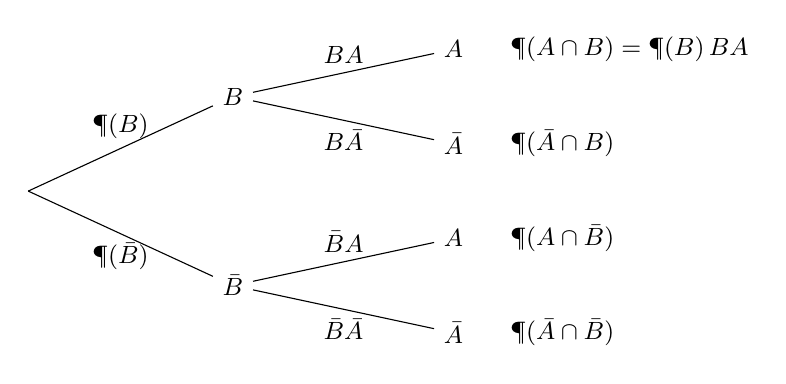
\begin{tikzpicture}[font=\small]
  \coordinate (root) at (0,0);
  \node (B)  at (2.6,1.2)  {$B$};
  \node (Bc) at (2.6,-1.2) {$\bar B$};
  \node (BA)  at (5.4,1.8)  {$A$};
  \node (BAc) at (5.4,0.6)  {$\bar A$};
  \node (BcA)  at (5.4,-0.6) {$A$};
  \node (BcAc) at (5.4,-1.8) {$\bar A$};
  \draw (root) -- (B)  node[midway, above] {$\P(B)$};
  \draw (root) -- (Bc) node[midway, below] {$\P(\bar B)$};
  \draw (B) -- (BA)   node[midway, above] {$\pcond{B}{A}$};
  \draw (B) -- (BAc)  node[midway, below] {$\pcond{B}{\bar A}$};
  \draw (Bc) -- (BcA)  node[midway, above] {$\pcond{\bar B}{A}$};
  \draw (Bc) -- (BcAc) node[midway, below] {$\pcond{\bar B}{\bar A}$};
  \node[anchor=west] at (6.0,1.8)  {$\P(A \cap B) = \P(B)\,\pcond{B}{A}$};
  \node[anchor=west] at (6.0,0.6)  {$\P(\bar A \cap B)$};
  \node[anchor=west] at (6.0,-0.6) {$\P(A \cap \bar B)$};
  \node[anchor=west] at (6.0,-1.8) {$\P(\bar A \cap \bar B)$};
\end{tikzpicture}

{\small 一个两层树状图：沿路径相乘，对各叶相加。
例如 $\P(A)$ 是第一个与第三个叶的
概率之和。}
\end{omfigure}

\begin{theorem}[贝叶斯公式]\label{thm:g12:condprob:bayes}
\index{贝叶斯公式}
设 $B_1, \dots, B_n$ 为如上所述的 $\Omega$ 划分，$A$ 为事件，
且 $\P(A) > 0$。则有
\[
\pcond{A}{B_j} =
\frac{\P(B_j)\,\pcond{B_j}{A}}{\sum_{i=1}^{n} \P(B_i)\,\pcond{B_i}{A}} .
\]
\end{theorem}

\begin{proof}
$\pcond{A}{B_j} = \frac{\P(A \cap B_j)}{\P(A)}$；分子由乘法公式展开，
分母由全概率公式展开。
\end{proof}

\begin{example}[筛查检验]\label{ex:g12:condprob:test}
某种疾病在总体中的患病率为 $1\%$。一种检验能以概率
$0.99$（灵敏度）检出该病，并以概率 $0.05$ 给出假阳性。
若检验结果为阳性，则实际患该病的概率为
\[
\frac{0.01 \times 0.99}{0.01\times0.99 + 0.99\times0.05}
= \frac{0.0099}{0.0099 + 0.0495} = \frac{1}{6} \approx 0.17 .
\]
尽管检验准确，六个阳性结果中有五个是假的 --- 因为
该病很罕见。混淆 $\pcond{A}{B}$ 与 $\pcond{B}{A}$ 是
\emph{检察官谬误}。
\end{example}

\begin{omfigure}
\begin{tikzpicture}[font=\small]
  \coordinate (root) at (0,0);
  \node (D)  at (2.6,1.2)  {$D$};
  \node (Dc) at (2.6,-1.2) {$\bar D$};
  \node (DT)  at (5.2,1.8)  {$T$};
  \node (DTc) at (5.2,0.6)  {$\bar T$};
  \node (DcT)  at (5.2,-0.6) {$T$};
  \node (DcTc) at (5.2,-1.8) {$\bar T$};
  \draw (root) -- (D)  node[midway, above] {$0.01$};
  \draw (root) -- (Dc) node[midway, below] {$0.99$};
  \draw (D) -- (DT)   node[midway, above] {$0.99$};
  \draw (D) -- (DTc)  node[midway, below] {$0.01$};
  \draw (Dc) -- (DcT)  node[midway, above] {$0.05$};
  \draw (Dc) -- (DcTc) node[midway, below] {$0.95$};
  \node[omThm, anchor=west] at (5.8,1.8)  {$0.0099$ \ （真阳性）};
  \node[anchor=west] at (5.8,0.6)  {$0.0001$};
  \node[omThm, anchor=west] at (5.8,-0.6) {$0.0495$ \ （假阳性）};
  \node[anchor=west] at (5.8,-1.8) {$0.9405$};
\end{tikzpicture}

{\small 筛查检验的树状图（$D$：患病，
$T$：检验阳性）。两个阳性叶（红色）的总权重为 $0.0594$，
其中假阳性贡献了六分之五。}
\end{omfigure}

\section{独立性}

\begin{definition}[独立事件]\label{def:g12:condprob:indep}
称两事件 $A$ 与 $B$ 为\emph{独立}\index{独立}，若
\[
\P(A \cap B) = \P(A)\,\P(B) .
\]
当 $\P(B) > 0$ 时，这等价于 $\pcond{B}{A} = \P(A)$：已知 $B$
不改变 $A$ 的概率。
\end{definition}

\begin{proposition}\label{prop:g12:condprob:indepcompl}
若 $A$ 与 $B$ 独立，则 $A$ 与 $\bar B$ 亦独立（$\bar A$ 与
$\bar B$）。
\end{proposition}

\begin{proof}
$\P(A \cap \bar B) = \P(A) - \P(A \cap B) = \P(A) - \P(A)\P(B)
= \P(A)\bigl(1 - \P(B)\bigr) = \P(A)\,\P(\bar B)$.
\end{proof}

\begin{remark}
不要把 \emph{独立}（$\P(A\cap B) = \P(A)\P(B)$）与
\emph{互斥}（$A \cap B = \varnothing$）。两个概率非零的
互斥事件永不独立：已知其中一个发生，
便能确定另一个未发生。
\end{remark}

\begin{definition}[独立重复试验]\label{def:g12:condprob:repet}
当一个试验重复进行 $n$ 次，使每次试验的结果
不影响其他各次试验时，指定结果序列的概率
等于各次概率之积。这正是
二项分布所依据的模型（见\cref{ch:g12:randvar}）。
\end{definition}

\section{练习}

\begin{exercise}[$\star$]\label{exo:g12:condprob:1}
从一副标准的 52 张扑克牌中抽取一张。求在
已知它为人头牌（杰克、皇后或国王）的条件下，它是国王的概率。“国王”与
“红心”两事件是否独立？
\end{exercise}

\begin{exercise}[$\star$]\label{exo:g12:condprob:2}
一个缸中有 5 个红球和 3 个蓝球。连续抽取两个球，
且为\emph{不放回}抽取。
\begin{enumerate}
  \item 画出概率树状图。
  \item 求两球均为红球的概率，以及
        第二次抽到红球的概率。
\end{enumerate}
\end{exercise}

\begin{exercise}[$\star$]\label{exo:g12:condprob:3}
掷两颗均匀的骰子。设 $A$ 为“点数之和为 $7$”，$B$ 为“第一颗
骰子点数为 $3$”，$C$ 为“点数之和为 $6$”。判断 $A$ 与 $B$
是否独立，再判断 $B$ 与 $C$ 是否独立。
\end{exercise}

\begin{exercise}[$\star\star$]\label{exo:g12:condprob:4}
某工厂有三台机器，分别生产总产量的 $50\%$、$30\%$ 和
$20\%$，次品率分别为 $1\%$、$2\%$ 和 $4\%$。
\begin{enumerate}
  \item 求产品中次品所占的比例。
  \item 随机抽取一件产品，它为次品。求它
        来自第三台机器的概率。
\end{enumerate}
\end{exercise}

\begin{exercise}[$\star\star$]\label{exo:g12:condprob:5}
在\cref{ex:g12:condprob:test}中，疾病患病率 $p$ 为多大时（而非
$1\%$）时，阳性结果意味着至少有 $90\%$ 的患病概率？解此
不等式并加以说明。
\end{exercise}

\begin{exercise}[$\star\star$]\label{exo:g12:condprob:6}
一枚有偏的硬币正面朝上的概率为 $p \in \intoo{0}{1}$。将该硬币
抛掷三次，各次抛掷相互独立。
\begin{enumerate}
  \item 求事件 $E$ = “恰好两次正面朝上”的概率。
  \item 当 $p$ 为何值时，$\P(E)$ 取得最大值？
\end{enumerate}
\end{exercise}

\begin{exercise}[$\star\star\star$]\label{exo:g12:condprob:7}
\emph{（蒙蒂·霍尔问题。）}奖品藏在三扇门中的一扇后。你先选
一扇门；主持人知道奖品的位置，他从其余两扇门中打开一扇
（若两扇均为空门，则随机选取），总是露出空门，
并提议你改选另一扇未打开的门。利用
贝叶斯公式，求改选时获胜的概率，以及不改选时
获胜的概率。
\end{exercise}

\begin{exercise}[$\star\star\star$]\label{exo:g12:condprob:8}
一信息信道传输比特。每个比特受噪声干扰而翻转的概率为
$\varepsilon = 0.1$，且各比特相互独立。为保护一个比特，将其
连续发送三次，并按多数表决译码。
\begin{enumerate}
  \item 求译码所得比特出错的概率。
  \item 接收到的码字为 $101$，求所发送的
        比特为 $1$ 的概率？（假设 $0$ 与 $1$ 等可能被发送。）
\end{enumerate}
\end{exercise}

\section{周末问题：医生、法官与垃圾邮件过滤器}

\begin{problem}[{周末问题 --- 贝叶斯公式对抗
基率谬误：为何 $99\,\%$ 的检测可能意味着 $2\,\%$，为何
百万分之一的匹配定不了任何人的罪，以及你的邮箱如何
“思考”}]
\label{pb:g12:condprob:1}
能检出 $99\,\%$ 病例的检测结果为阳性 ---
而真实患病概率低于 $2\,\%$。一份 DNA
图谱与百万分之一的人相符，被查出 --- 而
嫌疑人很可能是无辜的。两种说法均正确，
两者都曾被医生与法庭误判，而二者皆可由本章
的一条公式解决：贝叶斯公式
（\cref{thm:g12:condprob:bayes}）。本题先以瓮中摸球训练它，
再用于诊所、法庭与收件箱。

\medskip
\noindent\textbf{第一部分 --- 熟练运算。}
\begin{enumerate}
  \item 一枚均匀硬币决定选取瓮 I（$2$ 个红球，$1$ 个蓝球）或瓮 II
        （$1$ 个红球，$3$ 个蓝球），然后摸出一球。求
        $\P(\text{红})$，利用全概率公式
        （\cref{thm:g12:condprob:total}）。
  \item 已知所摸出的球为红球，求 $\P(\text{瓮 I} \mid
        \text{红})$。
  \item 掷一枚骰子：事件“偶数”与
        “$\leq 4$”是否相互独立
        （\cref{def:g12:condprob:indep}）？再问，“偶数”与
        “$\leq 3$”是否相互独立？
  \item 两个相互独立的烟雾报警器在火灾中各自触发的概率均为
        $0.9$。利用
        \cref{prop:g12:condprob:indepcompl}，求
        至少一个报警器触发的概率。
  \item 不放回地抽取两张牌，求
        $\P(\text{两张均为K})$，利用乘法法则
        （\cref{prop:g12:condprob:product}）。
\end{enumerate}

\medskip
\noindent\textbf{第二部分 --- 医生。}
某疾病的患病率为 $1$ 比 $1\,000$。该检测能检出
$99\,\%$ 的患者（灵敏度），但也会将 $5\,\%$ 的健康人
误判为阳性（假阳性）。
\begin{enumerate}[resume]
  \item 自然频数：设想有 $100\,000$ 人。其中
        患病者与健康者各有多少人？
        各组分别产生多少阳性结果，
        阳性结果总共多少？
  \item 由上述计数，求
        $\P(\text{患病} \mid \text{阳性})$。请先接受
        这一结果带来的冲击。
  \item 用贝叶斯公式重新计算，并检验
        两者是否一致。
  \item 在调查中，多数医生回答“约
        $99\,\%$”。请指出被混淆的两个条件概率，
        并解释为何极小的基率
        决定了真实的答案。
  \item 第二次独立的检测结果同样为阳性。
        更新：取 $1.9\,\%$ 为新的先验概率，求
        $\P(\text{患病} \mid \text{两次阳性})$。
        证据\emph{累积}起了什么作用？
  \item 若同一检测仅用于高风险人群，求 $\P(\text{患病} \mid \text{阳性})$，
        该群体的
        患病率为 $5\,\%$。由此推出关于
        罕见疾病大规模筛查的公共卫生教训。
\end{enumerate}

\medskip
\noindent\textbf{第三部分 --- 法官。}
\begin{enumerate}[resume]
  \item 案发现场的 DNA 图谱与百万人中的一人相符。
        嫌疑人经搜索一个数据库而被找到，该数据库
        包含全市 $10$ 百万居民，嫌疑人的图谱相符。预期
        全市有多少名无辜者会相符？仅凭这一相符结果，
        求 $\P(\text{无辜} \mid
        \text{相符})$ 的大致值为多少？
  \item 指出此谬误 --- 检察官引用的是哪一个概率，法庭
        需要的又是哪一个？ ---
        并说明它与第 9 题的确切对应关系。
  \item 独立性陷阱：同一家庭中的两起罕见悲剧
        曾被视为独立事件而相乘，得出“$73$ 百万分之一”，
        将二者视为独立，从而将一位无辜的母亲定罪
        （萨莉·克拉克案）。若两事件共享
        家庭风险因素，使得在第一事件发生的前提下，
        第二事件的概率是基率的 $5$ 倍，
        请重新估算其数量级 --- 并指出
        关于概率相乘的教训。
  \item 辩方同样可以耍花招：“十名无辜者会相符，所以
        该相符结果什么也证明不了”，忽略了其他一切证据。
        贝叶斯公式如何处理\emph{多条}证据，
        以及每位陪审员都应知道的
        那一句话是什么？
\end{enumerate}

\medskip
\noindent\textbf{第四部分 --- 垃圾邮件过滤器。}
\begin{enumerate}[resume]
  \item 你的邮件中有 $40\,\%$ 是垃圾邮件。单词“彩票”
        出现在 $15\,\%$ 的垃圾邮件和 $0.5\,\%$ 的正常邮件中。
        若一封邮件含有该词，计算
        $\P(\text{垃圾邮件} \mid \text{彩票})$。
  \item 纠错重复码
        （延续\cref{exo:g12:condprob:8}）：翻转概率为
        $\varepsilon = 0.1$，对\emph{五}份副本作多数译码，
        失败的概率是多少？
        与三份副本的码相比较。
  \item 一个比特穿过 $4$ 个相互独立的带噪中继，每个中继以
        概率 $0.1$ 将其翻转。该比特正确到达，当且仅当翻转次数为偶数。
        计算该概率两次：
        一次对二项式项求和，另一次
        用巧妙的公式
        $\frac{1 + (1 - 2\varepsilon)^4}{2}$。
  \item 真实的垃圾邮件过滤器将许多单词的证据相乘，
        仿佛它们相互独立（“朴素”贝叶斯）。这一假设
        对“中奖”和“彩票”这类单词不成立——
        而过滤器却仍然效果良好？
        （一两句话即可。）
  \item 终章 --- 贝叶斯公式作为信念的算术：先验
        $\times$ 似然，重新归一化，得后验。依次
        用一句话重述三个判决（诊所、法庭、收件箱），
        然后列出本题揭示的三个陷阱：
        遗忘基率、虚假的独立性，以及
        逐条阅读证据。
\end{enumerate}
\end{problem}
